\frontmatter

% Voorpagina met titel
\title{Efficient Implementations of\\ Attribute-based Credentials on Smart Cards}
\author{ir. Pim Vullers}

\maketitle

% Copyright informatie en ISBN (op achterzijde van de voorpagina)
%
% ISBN:
%   In het proefschrift dient in de regel een ISBN (Internationaal Standaard
%   Boeknummer) te worden aangebracht. U kunt deze aanvragen via internet op
%   http://www.isbn.nl/.
\thispagestyle{empty}

\noindent
The work in this thesis has been carried out while the author was employed at
the Radboud University Nijmegen, sponsored by Trans Link Systems / Open
Ticketing within the ``Applet-based e-ticketing'' project.

\vspace{146mm}

\noindent Typeset using \LaTeX \\\null

\noindent
\begin{tabular}{ll}
  ISBN & \dots \\
  NUR  & \dots \\
\end{tabular} \\\null

\noindent
\textcopyright\ Pim Vullers, 2010 \\\null

\begin{wrapfigure}{l}{40mm}
  \vspace{-5mm}
  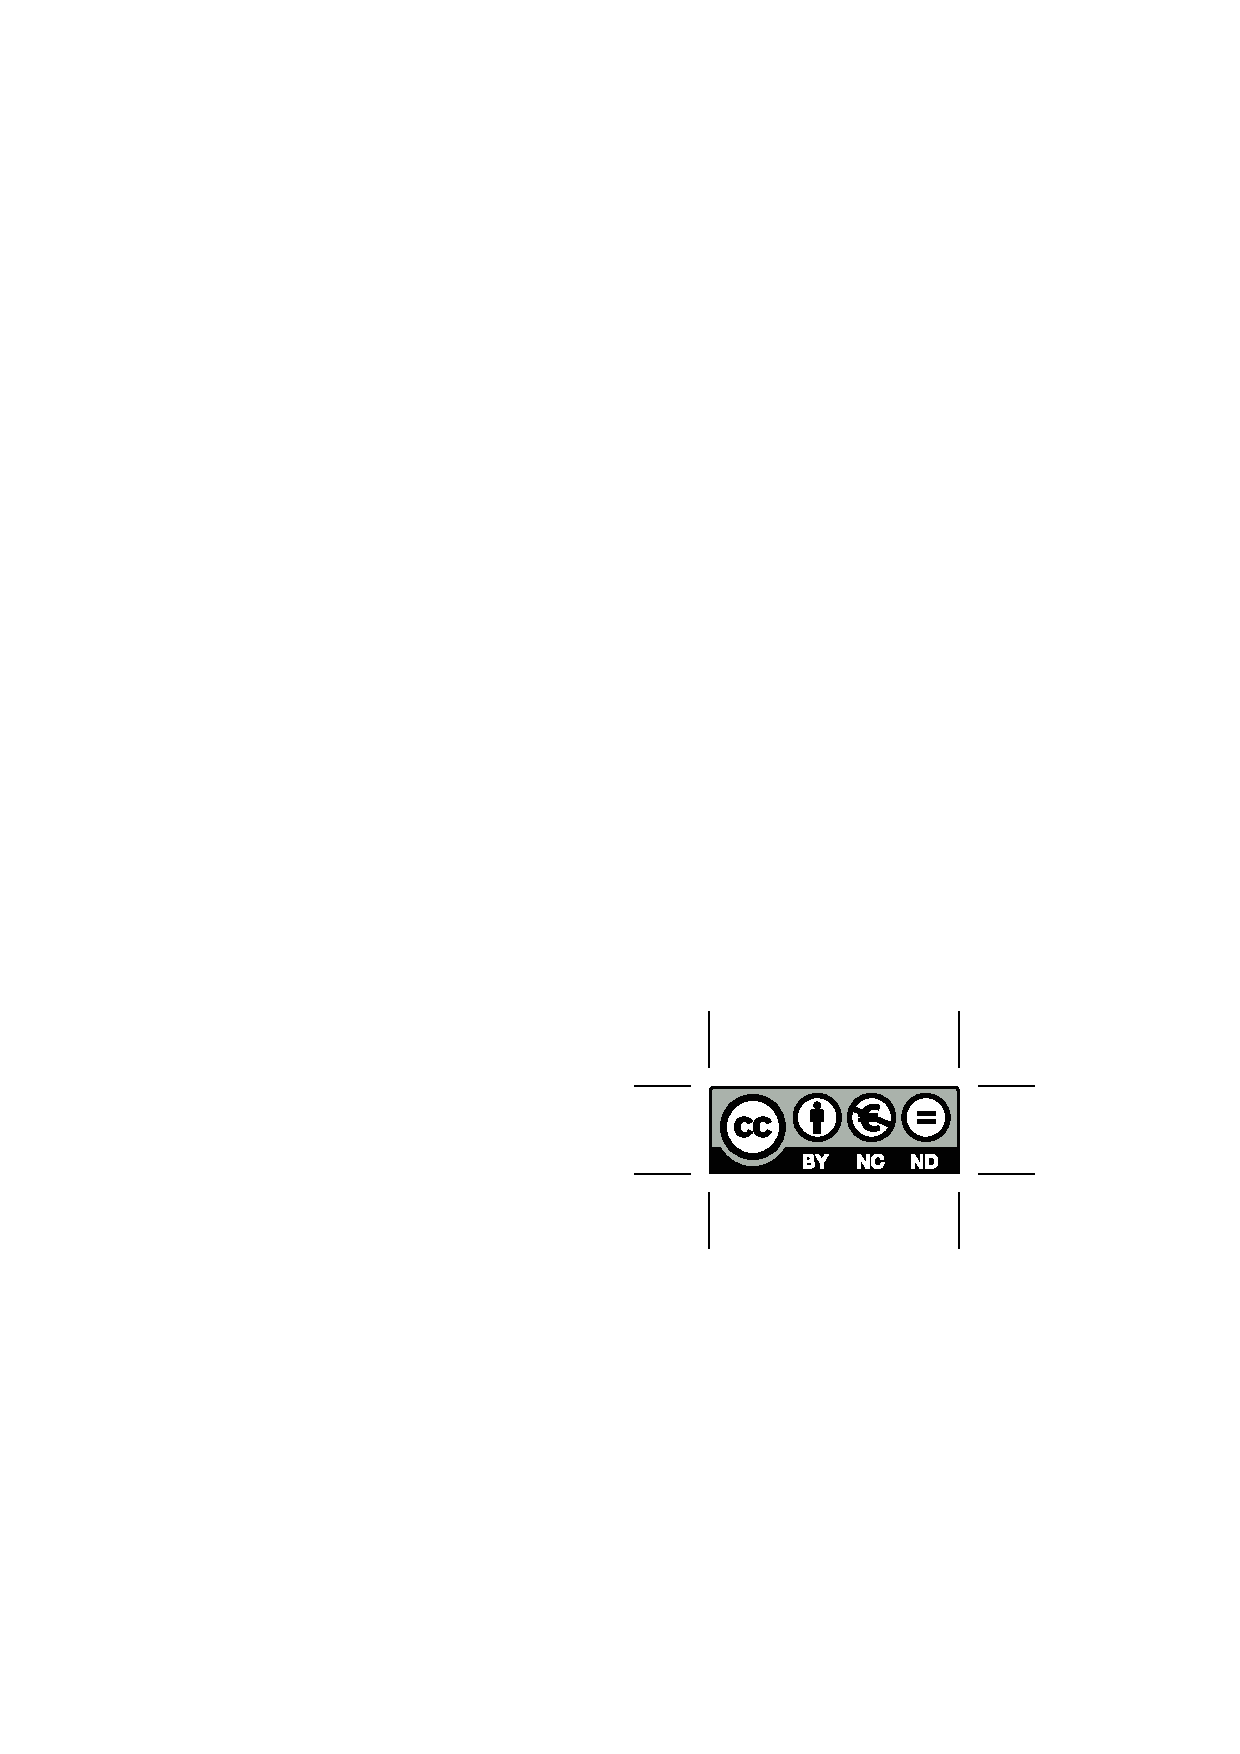
\includegraphics[scale=.94]{images/license}
  \vspace{-9mm}
\end{wrapfigure}

\noindent
This work is licensed under the Creative Commons Attribution-NonCommercial-NoDerivatives 4.0 International License. On-line available at:

\noindent
\url{http://creativecommons.org/licenses/by-nc-nd/4.0/}


% Verplichte titelpagina in het Nederlands
%
% De taal van het proefschrift:
%   Het proefschrift wordt geschreven in het Nederlands, of in het Engels, het
%   Frans, het Spaans of het Duits, of - met goedkeuring van de rector
%   magnificus in een andere taal. Indien het proefschrift in het Nederlands is
%   geschreven, worden daaraan een vertaling van de titel en een samenvatting
%   van de inhoud in het Engels bijgevoegd; desgewenst kan daarnaast ook een
%   samenvatting worden bijgevoegd in een andere taal naar keuze. Indien het
%   proefschrift niet in het Nederlands is geschreven, worden in elk geval de
%   titel en een samenvatting van de inhoud in het Nederlands en ten minste in
%   een van de hierboven genoemde talen toevoegd. De titelpagina is altijd in
%   het Nederlands, een titelpagina in een van bovengenoemde talen mag worden
%   toegevoegd. (Promotiereglement, pagina 25)
%
% Titelblad:
%   Het titelblad van het proefschrift wordt als volgt ingedeeld:
%    a. de titel;
%    b. de ondertitel (eventueel);
%    c. een wetenschappelijke proeve op het gebied van ......;
%    d. de volgende tekst:
%         Proefschrift ter verkrijging van de graad van doctor aan de Radboud
%         Universiteit Nijmegen op gezag van de rector magnificus, (naam),
%         volgens besluit van het College van Decanen in het openbaar te
%         verdedigen op (datum), om (tijd) uur precies door (voornamen voluit,
%         gevolgd door de achternaam) geboren op (geboortedatum) te
%         (geboorteplaats).;
%   aan de voet van de pagina: de naam van de uitgever en de plaats van uitgave.
%   (Promotiereglement, pagina 26)
%
% Achterzijde titelblad:
%   De naam van de promotor wordt vermeld op de achterzijde van het titelblad.
%   Zijn er meerdere promotores benoemd, dan dient uit de volgorde van de namen
%   van de promotores te blijken welke hoogleraar bij de voorbereiding van het
%   proefschrift het meest betrokken is geweest. Indien een copromotor is
%   benoemd dan wordt diens naam ook op de achterzijde van het titelblad vermeld
%   en wanneer er meerdere copromotores zijn benoemd dan dient eveneens uit de
%   volgorde van hun namen te blijken wie het meest bij de voorbereiding van het
%   proefschrift betrokken is geweest. Indien promotor(es) of copromotor(es) van
%   elders komen, dient de universiteit van herkomst te worden vermeld.
%   Op deze pagina worden tevens de namen vermeld van de leden van de
%   manuscriptcommissie. Indien een lid van de manuscriptcommissie van elders
%   komt, dient de universiteit of het instituut van herkomst te worden vermeld.
%   (Promotiereglement, pagina 26)
\thispagestyle{empty}

\begin{center}
  \textbf{\Large Applet-based e-Ticketing}\\[15mm]

  Een wetenschappelijke proeve op het gebied van de \\
  Natuurwetenschappen, Wiskunde en Informatica \\[15mm]

  \textsc{Proefschrift} \\[15mm]

  ter verkrijging van de graad van doctor \\
  aan de Radboud Universiteit Nijmegen \\
  op gezag van de rector magnificus, prof. mr. S.C.J.J. Kortmann, \\
  volgens besluit van het College van Decanen \\
  in het openbaar te verdedigen op \textbf{vrijdag 16 augustus 2013} \\
  om \textbf{..:.. uur} precies. \\[30mm]

  door \\[30mm]

  Pim Vullers \\[15mm]

  geboren op 20 juni 1986 \\
  te Venlo
\end{center}

\clearpage

\begin{flushleft}
  \thispagestyle{empty}

  \textbf{Promotor:} \\
  \indent Prof. dr. B.P.F. Jacobs \\[15mm]

  \textbf{Manuscriptcommissie:}
\end{flushleft}

% Verplichte samenvating in het Nederlands:
%
% Zie 'De taal van het proefschrift' hierboven
\chapter*{Samenvatting}
\addcontentsline{toc}{chapter}{Samenvatting}

We leven in een wereld waarin computers een steeds grotere rol spelen. Daarom 
wordt het alsmaar belangrijker om digitale entiteiten te identificeren. Om dit
te bereiken gebruiken veel bestaande systemen unieke herkenningspunten. Dit is
een eenvoudige oplossing, maar dit maakt het ook gemakkelijk om iemands 
handelingen te volgen. Een privacy-vriendelijk alternatief is om 
verificatiegegevens op basis van attributen te gebruiken voor authenticatie en
autorisatie. Zulke verificatiegegevens zijn een soort cryptografische container
voor attributen, ook wel gebruikerseigenschappen, welke gecertificeerd zijn 
door een autoriteit. Met behulp van deze attributen kan een gebruiker 
geauthentiseerd worden om toegang te krijgen tot bepaalde informatie of gebruik
te maken van een dienst door alleen de relevante gebruikerseigenschappen te 
delen.

In dit proefschrift bespreken we drie technologieën betreffende 
verificatiegegevens gebaseerd op attributen, waarvoor we efficiënte smartcard
implementaties hebben ontwikkeld. Deze technologieën zijn:

\paragraph{Self-blindable Credentials}
Deze verificatiegegevens zijn gebaseerd op elliptische kromme cryptografie met 
bilineaire paren. Deze technologie laat de terminal de berekeningen doen, wat 
een zeer compacte implementatie op de smartcard mogelijk maakt. Helaas is de 
ondersteuning voor elliptische kromme cryptografie beperkt tot de standaard 
algoritmes. Dit maakt de ontwikkeling van andere varianten op deze technologie
moeilijk. In vergelijking met de andere technologieën heeft de self-blindable 
credentials beperkte mogelijkheden.

\paragraph{U-Prove}
De uitgifte en verificatieprotocollen zijn respectievelijk gebaseerd op de 
blind signature scheme van Schnorr en de zero-knowledge proofs. Deze 
technologie biedt de snelste implementatie voor verificatie met attributen. 
Met betrekking tot privacy is er een groot probleem: U-Prove beschermt niet 
tegen het aan elkaar koppelen van meerdere verificatiesessies. Dit betekent
dat deze verificatiegegevens werken als een pseudoniem van de gebruiker.

\paragraph{Identity Mixer}
Deze technologie is gebaseerd op de signature scheme van Camenisch-Lysyanskaya,
welke een blind signature protocol bevat, dat gebruikt kan worden voor de 
uitgifte van de verificatiegegevens, en zero-knowledge proofs voor de 
verificatie van attributen. De prestaties van deze implementatie zijn niet de 
beste vergeleken met de andere, maar deze technologie biedt uitgebreide 
mogelijkheden en heeft een goede bescherming. Verificatiegegevens kunnen 
hierbij meerdere keren gebruikt worden zonder dat het traceerbaar wordt.

\paragraph{}
Het doel van het onderzoek was om efficiënte smartcard implementaties te maken 
voor verificatiegegevens op basis van attributen en



% Voorwoord in het Nederlands (hier vermelden dat de scriptie verder Engels is)
%
% Dankbetuigingen:
%   Personen en instellingen die ideele of materiele medewerking hebben verleend
%   aan de totstandkoming van het proefschrift of een onderdeel daarvan, kunnen
%   worden vermeld:
%    - in een voorbericht of op de achterzijde van de titelpagina indien de
%      medewerking op het gehele proefschrift betrekking heeft gehad;
%    - dan wel in een voetnoot op de eerste bladzijde van het desbetreffende
%      onderdeel indien het medewerking aan een specifiek onderdeel betreft.
\chapter*{Voorwoord}
\addcontentsline{toc}{chapter}{Voorwoord}

\cleardoublepage

% Titelpagina in het Engels
%
% Zie 'De taal van het proefschrift' hierboven.
\thispagestyle{empty}

\begin{center}
  ~ \\[25mm]

  \textbf{\Large Efficient Implementations of\\ Attribute-based Credentials on Smart Cards}\\[20mm]

  \textsc{Doctoral Thesis} \\[15mm]

  to obtain the degree of doctor \\
  from Radboud University Nijmegen \\
  on the authority of the Rector Magnificus, prof. dr. Th.L.M. Engelen, \\
  according to the decision of the Council of Deans \\
  to be defended in public on \textbf{Friday, November 28, 2014} \\
  at \textbf{10.30 hours}. \\[20mm]

  by \\[20mm]

  Pim Vullers \\[15mm]

  Born on June 20, 1986 \\
  in Venlo, The Netherlands
\end{center}

\clearpage

\thispagestyle{empty}

\noindent\textbf{Supervisor:} \\[2mm]
\indent\begin{tabular}{p{40mm}l}
  Prof. dr. B.P.F. Jacobs & \\
\end{tabular} \\[2mm]

\noindent\textbf{Doctoral Thesis Committee:} \\[2mm]
\indent\begin{tabular}{p{40mm}l}
  Prof. dr. E.R. Verheul     & \\
  Prof. dr. S. Mauw          & Universit\'{e} du Luxembourg, Luxembourg \\
  Prof. dr. ir. B. de Decker & KU Leuven, Belgium \\
  Dr. G. Neven               & IBM Research Z\"{u}rich, Switzerland \\
  Dr. ir. E. Poll            & \\
\end{tabular}


% Samenvatting in het Engels
\chapter*{Abstract}
\addcontentsline{toc}{chapter}{Abstract}

In a world where computers are involved in most aspects of our lives, it
becomes more and more important to digitally identify entities. To achieve 
this goal, many existing systems use unique identifiers. This is a simple
solution, but also makes it easy to trace the user's actions. A 
privacy-friendly alternative is to use attribute-based credentials as a 
basis for authentication and authorisation. Such credentials serve as a 
cryptographic container for attributes, that is, properties of the user,
which are certified by an authority. With these attributes the user can 
be authenticated to access a resource or receive a service solely on the 
properties that are relevant for that specific resource or service.

In this thesis we discuss three attribute-based credential technologies 
for which we have developed efficient smart card implementations. These 
technologies are:

\paragraph{Self-blindable Credentials}
These credentials are based on elliptic curve cryptography with bilinear 
pairings. This technology shifts the computational burden to the terminal 
which makes a very compact smart card implementation possible. 
Unfortunately the support for elliptic curve cryptography on smart cards 
is limited to standard algorithms, which made it hard to develop other 
variants of this technology. This results in a minimal feature set 
compared to the other technologies.

\paragraph{U-Prove}
The U-Prove issuance and verification protocols are, respectively, based 
on Schnorr's blind signature scheme and zero-knowledge proofs. This 
technology offers the fastest implementation for attribute verification. 
With respect to privacy there is only one important drawback: U-Prove 
does not protect against linking multiple verification sessions to each 
other. This means that these credentials basically act as a pseudonym for 
the user.

\paragraph{Identity Mixer}
This technology is based on the Camenisch-Lysyanskaya signature scheme 
which provides a blind signature protocol, which can be used for 
credential issuance, and zero-knowledge proofs for attribute verification. 
The performance of this implementation is not the best among these 
technologies, but this technology provides a broad feature set and offers 
proper unlinkability. This makes it possible to use a credential 
multiple times without becoming traceable.

\paragraph{}
The goal of the research presented in this thesis has been to \emph{develop 
efficient smart card implementations of attribute-based credentials} and 
\emph{compare various cryptographic systems for attribute-based credentials}. 
This has resulted in a detailed description and discussion of the
technologies listed above and the smart card implementations\footnote{The
source code of these implementations is available at 
\url{http://github.com/pimvullers/}.} for each of these technologies, which are
the most efficient implementations at the time of writing.

Furthermore, the successful development of these implementations laid
the foundation for the IRMA project. This is an on-going research and
development project focusing on attribute-based credentials and their
use in practice. For more information concerning the IRMA project,
please visit \url{https://www.irmacard.org/}.


% Voorwoord in het Engels
%
% Zie 'Dankbetuigingen' hierboven.
\chapter*{Preface}
\addcontentsline{toc}{chapter}{Preface}

[TODO: Preface in English.]

% Inhoudsopgave
\tableofcontents

%\listoffigures
%\listoftables
%\listofalgorithms